\documentclass[sigconf,review, anonymous]{acmart}
\acmConference[ESEC/FSE 2020]{The 28th ACM Joint European Software Engineering Conference and Symposium on the Foundations of Software Engineering}{8 - 13 November, 2020}{Sacramento, California, United States}

%\documentclass[12pt, letterpaper, twoside, twocolumn]{article}
\usepackage[utf8]{inputenc}

\title{First document}
%\author{Hubert Farnsworth \thanks{funded by the Overleaf team}}
\date{February 2017}

\usepackage{graphicx}
\graphicspath{ {images/} }
%\usepackage{lineno}
\usepackage[switch]{lineno}
\begin{document}
\maketitle
First document. This is a simple example, with no extra parameters or packages included.
\linenumbers
\bibliographystyle{IEEEtran}

\begin{abstract}
This is a simple paragraph at the beginning of the 
document. A brief introduction about the main subject.
\end{abstract}

%test the format Bold, italics and underlining
Some of the \textbf{greatest}
discoveries in \underline{science} 
were made by \textbf{\textit{accident}}.

Some of the greatest \emph{discoveries} 
in science 
were made by accident.

\textit{Some of the greatest \emph{discoveries} 
in science 
were made by accident.}

\textbf{Some of the greatest \emph{discoveries} 
in science 
were made by accident.}
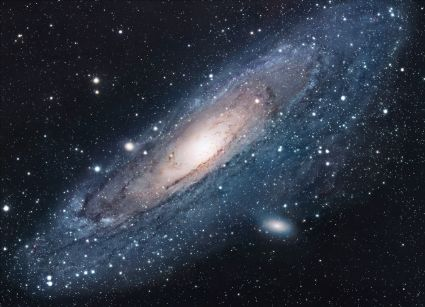
\includegraphics{universe}
\begin{figure}[h]
    \centering
    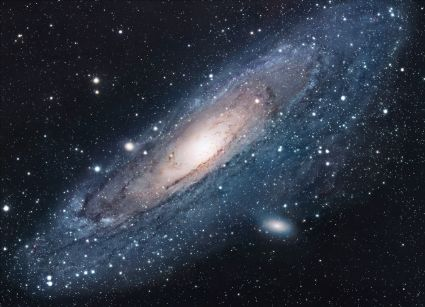
\includegraphics[width=0.25\textwidth]{universe}
    \caption{a nice plot}
    \label{fig:mesh1}
\end{figure}

\begin{enumerate}
  \item This is the first entry in our list
  \item The list numbers increase with each entry we add
\end{enumerate}
\begin{center}
 \begin{tabular}{||c c c c||} 
 \hline
 Col1 & Col2 & Col2 & Col3 \\ [0.5ex] 
 \hline\hline
 1 & 6 & 87837 & 787 \\ 
 \hline
 2 & 7 & 78 & 5415 \\
 \hline
 3 & 545 & 778 & 7507 \\
 \hline
 4 & 545 & 18744 & 7560 \\
 \hline
 5 & 88 & 788 & 6344 \\ [1ex] 
 \hline
\end{tabular}
\end{center}
\end{document}